\chapter{几何空间中的平面与直线}

% SOURCE_PDF_PAGE 238

\hypertarget{source-p238}{}
\phantomsection\addcontentsline{toc}{section}{5.1 竞赛要点与难点}
\phantomsection\addcontentsline{toc}{section}{5.2 范例解析与精讲}

在几何空间中引进坐标系之后，平面与直线分别由一个和两个线性方程确定，把向量
法与坐标法结合起来研究平面与平面、直线与直线、平面与直线的关系和性质，主要包括
它们的仿射性质和度量性质.
M 竞赛要点与难点问
1.平面方程、直线方程的各种形式，方程中各有关字母的意义.
2. 从决定平面和直线的几何条件出发，选用适当方法建立平面、直线方程.
3. 根据平面和直线的方程，判定平面与平面、直线与直线、平面与直线间的位置关系.
4 . 根据平面和直线的方程及点的坐标判定有关点、平面、直线之间的位置关系，计
算它们之间的距离与交角等; 求两异面直线的公垂线方程.
\section*{5.2 范例解析与精讲}
国也型卢竹林也方程护的程
确定一个平面方程有几种方式:例如经过不共线的三点确定一个平面; 经过一条直线
和直线外的一点确定一个平面; 经过两条相交的直线确定一个平面; 经过两条不重合的平
行直线确定一个平面;等等.表示平面的方程通常有参数方程和一般方程.
1.平面的参数方程
\sourceblock{450.00}{images-full/p238-d001.png}
2. 平面的一般方程
设平面\allowbreak{}\raisebox{-1.68pt}{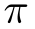
\includegraphics[width=9.60pt]{images-full/p238-i000.png}}\allowbreak{}经过点\allowbreak{}\raisebox{-2.88pt}{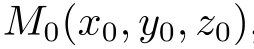
\includegraphics[width=71.69pt]{images-full/p238-i001.png}}\allowbreak{}，且与平面\allowbreak{}\raisebox{-1.68pt}{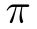
\includegraphics[width=10.17pt]{images-full/p238-i002.png}}\allowbreak{}垂直的方向(法方向)为\allowbreak{}\raisebox{-2.88pt}{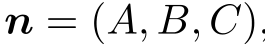
\includegraphics[width=74.41pt]{images-full/p238-i003.png}}\allowbreak{}，
则对平面\allowbreak{}\raisebox{-1.56pt}{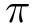
\includegraphics[width=10.17pt]{images-full/p238-i004.png}}\allowbreak{}上任意一点\allowbreak{}\raisebox{-3.00pt}{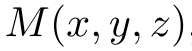
\includegraphics[width=54.00pt]{images-full/p238-i005.png}}\allowbreak{}，有\allowbreak{}\raisebox{-3.96pt}{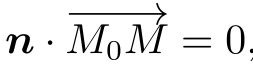
\includegraphics[width=71.40pt]{images-full/p238-i006.png}}\allowbreak{}，即


% SOURCE_PDF_PAGE 239

\hypertarget{source-p239}{}
\sourceblock{292.10}{images-full/p239-d000.png}
其中\allowbreak{}\raisebox{-2.76pt}{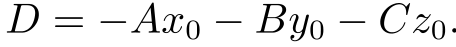
\includegraphics[width=128.69pt]{images-full/p239-i000.png}}\allowbreak{}. 称(5.2.2) 式为平面\allowbreak{}\raisebox{-1.56pt}{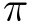
\includegraphics[width=9.60pt]{images-full/p239-i001.png}}\allowbreak{}的一般方程.
【注5.2.1 】从(5.2.2) 式可知当平面\allowbreak{}\raisebox{-1.68pt}{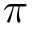
\includegraphics[width=9.60pt]{images-full/p239-i002.png}}\allowbreak{} 经过原点时，\allowbreak{}\raisebox{-2.64pt}{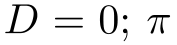
\includegraphics[width=49.72pt]{images-full/p239-i003.png}}\allowbreak{}r平行于$z$ 轴当且仅
当\allowbreak{}\raisebox{-2.76pt}{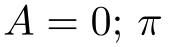
\includegraphics[width=47.46pt]{images-full/p239-i005.png}}\allowbreak{}平行于$u$ 轴当且仅当\allowbreak{}\raisebox{-2.64pt}{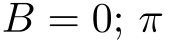
\includegraphics[width=48.02pt]{images-full/p239-i007.png}}\allowbreak{}r平行于$z$轴当且仅当\allowbreak{}\raisebox{-2.40pt}{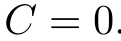
\includegraphics[width=33.88pt]{images-full/p239-i009.png}}\allowbreak{}
\par\medskip\noindent\textbf{【例5.2.1 】(第十四届全国初赛第二次补赛题)设在空间直角坐标系中三角形\allowbreak{}\raisebox{-2.40pt}{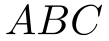
\includegraphics[width=30.51pt]{images-full/p239-i010.png}}\allowbreak{}}
的三个顶点分别为\allowbreak{}\raisebox{-3.00pt}{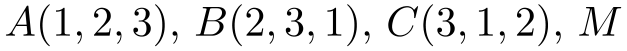
\includegraphics[width=176.84pt]{images-full/p239-i011.png}}\allowbreak{}为三角形\allowbreak{}\raisebox{-2.28pt}{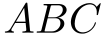
\includegraphics[width=29.94pt]{images-full/p239-i012.png}}\allowbreak{} 的三条中线的交点
(重心).求过点$M$ 的平面方程，使得该平面与三角形\allowbreak{}\raisebox{-2.28pt}{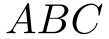
\includegraphics[width=30.51pt]{images-full/p239-i014.png}}\allowbreak{} 垂直，且与直线\allowbreak{}\raisebox{-2.28pt}{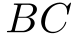
\includegraphics[width=22.03pt]{images-full/p239-i015.png}}\allowbreak{} 平行.
解重心$M$ 的坐标为
\sourceblock{132.77}{images-full/p239-d001.png}
\sourceblock{320.35}{images-full/p239-d002.png}
所以，三角形\allowbreak{}\raisebox{-2.28pt}{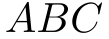
\includegraphics[width=30.51pt]{images-full/p239-i017.png}}\allowbreak{}所在平面的法向量为
\sourceblock{206.79}{images-full/p239-d003.png}
设所求平面的法向量为\allowbreak{}\raisebox{-3.00pt}{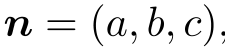
\includegraphics[width=63.22pt]{images-full/p239-i018.png}}\allowbreak{}，由题设可知\allowbreak{}\raisebox{-3.00pt}{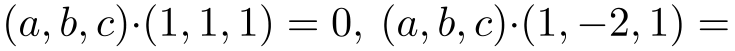
\includegraphics[width=204.00pt]{images-full/p239-i019.png}}\allowbreak{}
0，即\allowbreak{}\raisebox{-2.64pt}{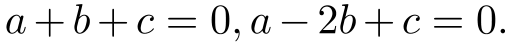
\includegraphics[width=142.51pt]{images-full/p239-i020.png}}\allowbreak{} 由此得\allowbreak{}\raisebox{-3.00pt}{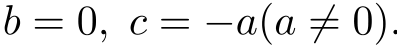
\includegraphics[width=111.96pt]{images-full/p239-i021.png}}\allowbreak{} 于是，所求平面的方程为
\sourceblock{180.80}{images-full/p239-d004.png}
即
\sourceblock{54.80}{images-full/p239-d005.png}
\par\medskip\noindent\textbf{【例5.2.2 】求过\allowbreak{}\raisebox{-3.00pt}{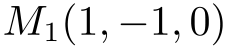
\includegraphics[width=64.97pt]{images-full/p239-i022.png}}\allowbreak{} 与\allowbreak{}\raisebox{-3.00pt}{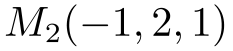
\includegraphics[width=65.54pt]{images-full/p239-i023.png}}\allowbreak{} 两点，而且平行于$u$轴的平面方程.}
解设所求平面的一般方程为
\sourceblock{127.69}{images-full/p239-d006.png}
由于平面平行于\allowbreak{}\raisebox{-2.16pt}{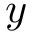
\includegraphics[width=9.04pt]{images-full/p239-i025.png}}\allowbreak{}轴，所以\allowbreak{}\raisebox{-2.76pt}{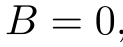
\includegraphics[width=34.23pt]{images-full/p239-i026.png}}\allowbreak{}，又困为平面经过\allowbreak{}\raisebox{-2.76pt}{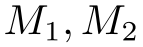
\includegraphics[width=40.11pt]{images-full/p239-i027.png}}\allowbreak{} 两点，所以
\sourceblock{272.33}{images-full/p239-d007.png}
\sourceblock{114.13}{images-full/p239-d008.png}
即
\sourceblock{77.97}{images-full/p239-d009.png}
为所求平面


% SOURCE_PDF_PAGE 240

\hypertarget{source-p240}{}
\par\medskip\noindent\textbf{【例5.2.3 】求垂直于平面\allowbreak{}\raisebox{-2.76pt}{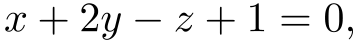
\includegraphics[width=100.24pt]{images-full/p240-i000.png}}\allowbreak{}，且经过$z$ 轴的平面方程.}
解设所求平面\allowbreak{}\raisebox{-1.68pt}{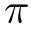
\includegraphics[width=9.60pt]{images-full/p240-i002.png}}\allowbreak{}的方程为
\sourceblock{127.69}{images-full/p240-d000.png}
平面\allowbreak{}\raisebox{-1.68pt}{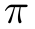
\includegraphics[width=9.60pt]{images-full/p240-i003.png}}\allowbreak{}的法向量\allowbreak{}\raisebox{-2.88pt}{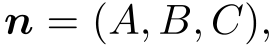
\includegraphics[width=76.75pt]{images-full/p240-i004.png}}\allowbreak{}由题意，作与己知平面垂直表明\allowbreak{}\raisebox{-2.52pt}{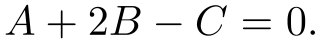
\includegraphics[width=88.69pt]{images-full/p240-i006.png}}\allowbreak{}由于
\allowbreak{}\raisebox{-1.68pt}{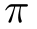
\includegraphics[width=10.17pt]{images-full/p240-i007.png}}\allowbreak{}经过$z$轴，则有\allowbreak{}\raisebox{-2.28pt}{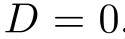
\includegraphics[width=35.11pt]{images-full/p240-i009.png}}\allowbreak{}，而且\allowbreak{}\raisebox{-2.88pt}{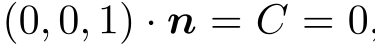
\includegraphics[width=105.72pt]{images-full/p240-i010.png}}\allowbreak{}，因此得到\allowbreak{}\raisebox{-2.28pt}{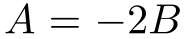
\includegraphics[width=52.34pt]{images-full/p240-i011.png}}\allowbreak{}. 于是，所求平
面\allowbreak{}\raisebox{-1.56pt}{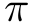
\includegraphics[width=10.17pt]{images-full/p240-i012.png}}\allowbreak{}满足
\sourceblock{88.70}{images-full/p240-d001.png}
即
\sourceblock{60.45}{images-full/p240-d002.png}
\par\medskip\noindent\textbf{【例5.2.4 】求过点\allowbreak{}\raisebox{-2.88pt}{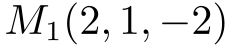
\includegraphics[width=64.97pt]{images-full/p240-i013.png}}\allowbreak{} 与\allowbreak{}\raisebox{-3.00pt}{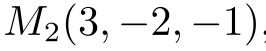
\includegraphics[width=74.73pt]{images-full/p240-i014.png}}\allowbreak{}，且垂直于平面\allowbreak{}\raisebox{-2.76pt}{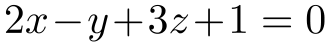
\includegraphics[width=93.79pt]{images-full/p240-i015.png}}\allowbreak{}}
的平面方程.
解设所求平面\allowbreak{}\raisebox{-1.68pt}{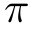
\includegraphics[width=9.60pt]{images-full/p240-i016.png}}\allowbreak{}的方程为
\sourceblock{127.69}{images-full/p240-d003.png}
\sourceblock{320.35}{images-full/p240-d004.png}
\sourceblock{151.98}{images-full/p240-d005.png}
\sourceblock{284.19}{images-full/p240-d006.png}
困县如何价低制其系
\par\noindent (1) 设两个平面的方程为
\sourceblock{172.32}{images-full/p240-d007.png}
\sourceblock{286.45}{images-full/p240-d008.png}


% SOURCE_PDF_PAGE 241

\hypertarget{source-p241}{}
\sourceblock{192.10}{images-full/p241-d000.png}
\sourceblock{290.41}{images-full/p241-d001.png}
的夹角为
\sourceblock{366.12}{images-full/p241-d002.png}
\par\noindent (3) 设\allowbreak{}\raisebox{-3.00pt}{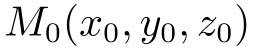
\includegraphics[width=71.19pt]{images-full/p241-i000.png}}\allowbreak{})为平面\allowbreak{}\raisebox{-2.76pt}{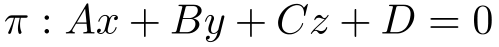
\includegraphics[width=140.68pt]{images-full/p241-i001.png}}\allowbreak{} 外一点，则点\allowbreak{}\raisebox{-2.64pt}{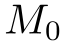
\includegraphics[width=18.64pt]{images-full/p241-i002.png}}\allowbreak{} 到\allowbreak{}\raisebox{-1.68pt}{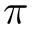
\includegraphics[width=9.60pt]{images-full/p241-i003.png}}\allowbreak{} 的距
\sourceblock{303.97}{images-full/p241-d003.png}
\sourceblock{283.63}{images-full/p241-d004.png}
\sourceblock{284.19}{images-full/p241-d005.png}
\sourceblock{290.41}{images-full/p241-d006.png}
\sourceblock{172.32}{images-full/p241-d007.png}
\sourceblock{168.93}{images-full/p241-d008.png}
\sourceblock{346.91}{images-full/p241-d009.png}
\sourceblock{124.86}{images-full/p241-d010.png}
其中\allowbreak{}\raisebox{-2.88pt}{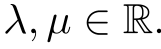
\includegraphics[width=45.26pt]{images-full/p241-i004.png}}\allowbreak{} 求\allowbreak{}\raisebox{-2.04pt}{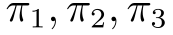
\includegraphics[width=48.59pt]{images-full/p241-i005.png}}\allowbreak{}交于一点的条件，并在它们交于一点时，求出交点的坐标.


% SOURCE_PDF_PAGE 242

\hypertarget{source-p242}{}
\sourceblock{253.12}{images-full/p242-d000.png}
设其系数矩阵为\allowbreak{}\raisebox{-2.76pt}{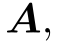
\includegraphics[width=15.82pt]{images-full/p242-i000.png}}\allowbreak{}经计算可得其系数行列式
\sourceblock{237.86}{images-full/p242-d001.png}
于是，当\allowbreak{}\raisebox{-2.76pt}{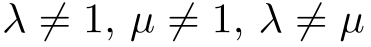
\includegraphics[width=104.52pt]{images-full/p242-i001.png}}\allowbreak{} 时，\allowbreak{}\raisebox{-2.76pt}{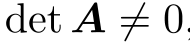
\includegraphics[width=53.27pt]{images-full/p242-i002.png}}\allowbreak{}，此时三个平面交于一点当三个平面交于一
点时，我们可得交点
\sourceblock{302.27}{images-full/p242-d002.png}
\par\medskip\noindent\textbf{【例5.2.6 】求两个相交平面\allowbreak{}\raisebox{-2.76pt}{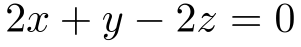
\includegraphics[width=84.75pt]{images-full/p242-i003.png}}\allowbreak{} 和\allowbreak{}\raisebox{-2.76pt}{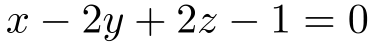
\includegraphics[width=105.65pt]{images-full/p242-i004.png}}\allowbreak{} 的二面角的}
平分面方程.
解设\allowbreak{}\raisebox{-3.00pt}{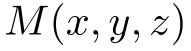
\includegraphics[width=53.67pt]{images-full/p242-i005.png}}\allowbreak{} 是平分面上任意一点，则有
\sourceblock{179.10}{images-full/p242-d003.png}
由此可得
\sourceblock{179.67}{images-full/p242-d004.png}
于是得到两个平面
\sourceblock{105.09}{images-full/p242-d005.png}
和
\sourceblock{80.79}{images-full/p242-d006.png}
\par\medskip\noindent\textbf{【例5.2.7】设原点\allowbreak{}\raisebox{-3.00pt}{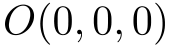
\includegraphics[width=48.59pt]{images-full/p242-i006.png}}\allowbreak{} 到平面}
\sourceblock{79.10}{images-full/p242-d007.png}
的距离为\allowbreak{}\raisebox{-2.76pt}{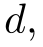
\includegraphics[width=11.86pt]{images-full/p242-i007.png}}\allowbreak{}求$d$ 与\allowbreak{}\raisebox{-2.76pt}{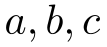
\includegraphics[width=29.94pt]{images-full/p242-i009.png}}\allowbreak{}之间的关系.
解利用点到平面的距离公式可得
\sourceblock{309.62}{images-full/p242-d008.png}


% SOURCE_PDF_PAGE 243

\hypertarget{source-p243}{}
园也型主共指导晶来
空间中经过同一直线$L$ 的所有平面构成的集合称为以$L$ 为轴的共轴平面束.
设有两个平面\allowbreak{}\raisebox{-2.88pt}{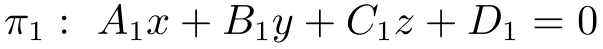
\includegraphics[width=170.06pt]{images-full/p243-i002.png}}\allowbreak{} 和\allowbreak{}\raisebox{-2.88pt}{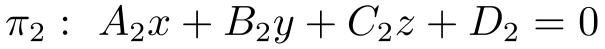
\includegraphics[width=170.63pt]{images-full/p243-i003.png}}\allowbreak{}
交于一条直线\allowbreak{}\raisebox{-2.64pt}{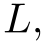
\includegraphics[width=12.99pt]{images-full/p243-i004.png}}\allowbreak{}则以$L$ 为轴的平面束的方程为
\sourceblock{311.88}{images-full/p243-d000.png}
其中μ ，ν 是不全为零的任意实数.
\sourceblock{257.07}{images-full/p243-d001.png}
并且与平面
\sourceblock{92.66}{images-full/p243-d002.png}
垂直的平面方程.
解考虑过所给直线的平面束方程
\sourceblock{228.82}{images-full/p243-d003.png}
即
\sourceblock{272.33}{images-full/p243-d004.png}
由题意可知，\allowbreak{}\raisebox{-2.88pt}{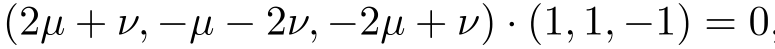
\includegraphics[width=218.56pt]{images-full/p243-i006.png}}\allowbreak{}，可得\allowbreak{}\raisebox{-2.76pt}{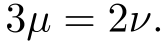
\includegraphics[width=45.15pt]{images-full/p243-i007.png}}\allowbreak{} 代入平面束可得
\sourceblock{107.35}{images-full/p243-d005.png}
\par\medskip\noindent\textbf{【例5.2.9 】(第十二届全国初赛补赛题)在空间直角坐标系\allowbreak{}\raisebox{-2.76pt}{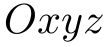
\includegraphics[width=30.51pt]{images-full/p243-i008.png}}\allowbreak{} 中，设\allowbreak{}\raisebox{-3.00pt}{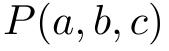
\includegraphics[width=47.46pt]{images-full/p243-i009.png}}\allowbreak{}}
为第一卦限中的点(即\allowbreak{}\raisebox{-2.88pt}{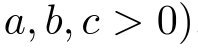
\includegraphics[width=55.74pt]{images-full/p243-i010.png}}\allowbreak{}，过点$P$ 的平面\allowbreak{}\raisebox{-1.68pt}{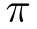
\includegraphics[width=10.17pt]{images-full/p243-i012.png}}\allowbreak{}分别交$z$ 轴、$u$ 轴和$z$ 轴的正半轴
于点\allowbreak{}\raisebox{-2.76pt}{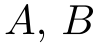
\includegraphics[width=28.25pt]{images-full/p243-i016.png}}\allowbreak{} 和$C$，并且$P$ 恰为三角形\allowbreak{}\raisebox{-2.40pt}{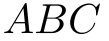
\includegraphics[width=30.51pt]{images-full/p243-i019.png}}\allowbreak{} 的重心.求平面\allowbreak{}\raisebox{-1.56pt}{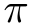
\includegraphics[width=9.60pt]{images-full/p243-i020.png}}\allowbreak{}的方程.
解设\allowbreak{}\raisebox{-3.00pt}{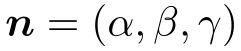
\includegraphics[width=67.80pt]{images-full/p243-i021.png}}\allowbreak{} 为所求平面\allowbreak{}\raisebox{-1.56pt}{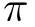
\includegraphics[width=9.60pt]{images-full/p243-i022.png}}\allowbreak{}的法向量，则\allowbreak{}\raisebox{-1.56pt}{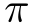
\includegraphics[width=10.17pt]{images-full/p243-i023.png}}\allowbreak{}的方程可写为
\sourceblock{320.92}{images-full/p243-d006.png}
由于平面\allowbreak{}\raisebox{-1.56pt}{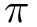
\includegraphics[width=10.17pt]{images-full/p243-i024.png}}\allowbreak{}与三个坐标轴的正半轴相交，故可设\allowbreak{}\raisebox{-2.76pt}{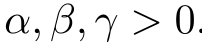
\includegraphics[width=56.79pt]{images-full/p243-i025.png}}\allowbreak{} 于是三个交点为
\sourceblock{413.01}{images-full/p243-d007.png}
\sourceblock{362.16}{images-full/p243-d008.png}


% SOURCE_PDF_PAGE 244

\hypertarget{source-p244}{}
代入方程(5.2.3) 并整理，得到平面\allowbreak{}\raisebox{-1.56pt}{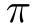
\includegraphics[width=10.17pt]{images-full/p244-i000.png}}\allowbreak{}的方程为
\sourceblock{434.48}{images-full/p244-d000.png}
\sourceblock{450.00}{images-full/p244-d001.png}
方程.
分析本题关键在于利用己知条件确定$Z$在点\allowbreak{}\raisebox{-2.64pt}{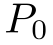
\includegraphics[width=14.69pt]{images-full/p244-i002.png}}\allowbreak{}的切平面的法向量.
解对等式\allowbreak{}\raisebox{-3.24pt}{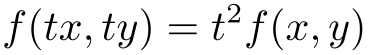
\includegraphics[width=104.52pt]{images-full/p244-i003.png}}\allowbreak{} 两边关于$t$求导，得
\sourceblock{204.53}{images-full/p244-d002.png}
\sourceblock{311.31}{images-full/p244-d003.png}
代入点\allowbreak{}\raisebox{-3.00pt}{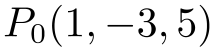
\includegraphics[width=61.02pt]{images-full/p244-i005.png}}\allowbreak{} 的坐标，得
\sourceblock{184.19}{images-full/p244-d004.png}
\sourceblock{450.00}{images-full/p244-d005.png}
\sourceblock{107.91}{images-full/p244-d006.png}
国也型四直制卢的程抑制程
1.直线的标准方程
直线$L$ 经过点\allowbreak{}\raisebox{-2.88pt}{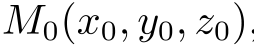
\includegraphics[width=71.35pt]{images-full/p244-i007.png}}\allowbreak{}，方向向量为\allowbreak{}\raisebox{-3.00pt}{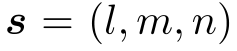
\includegraphics[width=66.67pt]{images-full/p244-i008.png}}\allowbreak{} 的标准方程(也称为对称式
方程)为
\sourceblock{298.32}{images-full/p244-d007.png}
\sourceblock{432.79}{images-full/p244-d008.png}


% SOURCE_PDF_PAGE 245

\hypertarget{source-p245}{}
3. 直线的参数方程
\sourceblock{432.79}{images-full/p245-d000.png}
设\allowbreak{}\raisebox{-3.00pt}{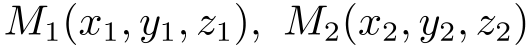
\includegraphics[width=149.86pt]{images-full/p245-i000.png}}\allowbreak{} 是直线$L$上不同的两点，则直线经过点\allowbreak{}\raisebox{-2.76pt}{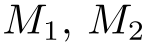
\includegraphics[width=42.37pt]{images-full/p245-i002.png}}\allowbreak{} 的
\sourceblock{305.66}{images-full/p245-d001.png}
5. 直线的一般方程化为标准方程
\sourceblock{334.48}{images-full/p245-d002.png}
\sourceblock{320.92}{images-full/p245-d003.png}
\sourceblock{327.13}{images-full/p245-d004.png}
所以直线$L$经过点\allowbreak{}\raisebox{-3.00pt}{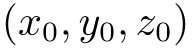
\includegraphics[width=54.24pt]{images-full/p245-i004.png}}\allowbreak{} 以\allowbreak{}\raisebox{-1.68pt}{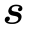
\includegraphics[width=8.47pt]{images-full/p245-i005.png}}\allowbreak{} 为方向向量的标准方程为
\sourceblock{184.75}{images-full/p245-d005.png}
\par\medskip\noindent\textbf{【例5.2.11 】把直线的一般方程}
\sourceblock{138.99}{images-full/p245-d006.png}
化为标准方程


% SOURCE_PDF_PAGE 246

\hypertarget{source-p246}{}
解直线$L$ 的方向向量为
\sourceblock{413.01}{images-full/p246-d000.png}
\sourceblock{267.24}{images-full/p246-d001.png}
垂直相交的直线的标准方程.
\sourceblock{450.00}{images-full/p246-d002.png}
\sourceblock{202.83}{images-full/p246-d003.png}
于是，设点\allowbreak{}\raisebox{-3.00pt}{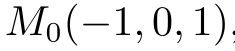
\includegraphics[width=66.07pt]{images-full/p246-i001.png}}\allowbreak{}，由题意则有
\sourceblock{354.82}{images-full/p246-d004.png}
\sourceblock{450.00}{images-full/p246-d005.png}
\sourceblock{104.52}{images-full/p246-d006.png}
\sourceblock{450.00}{images-full/p246-d007.png}
\par\noindent (1) 求连接$N$ 与$A$ 两点的直线方程;
\par\noindent (2) 求\allowbreak{}\raisebox{-2.76pt}{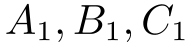
\includegraphics[width=53.67pt]{images-full/p246-i004.png}}\allowbreak{}三点的坐标;
\par\noindent (3) 给定点\allowbreak{}\raisebox{-3.00pt}{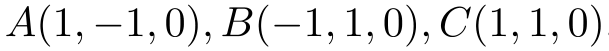
\includegraphics[width=171.84pt]{images-full/p246-i005.png}}\allowbreak{}，求四面体\allowbreak{}\raisebox{-2.64pt}{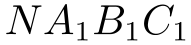
\includegraphics[width=53.67pt]{images-full/p246-i006.png}}\allowbreak{} 的体积.


% SOURCE_PDF_PAGE 247

\hypertarget{source-p247}{}
解(1) 根据直线的两点式方程，直接得连接\allowbreak{}\raisebox{-2.76pt}{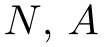
\includegraphics[width=29.38pt]{images-full/p247-i000.png}}\allowbreak{}两点的直线方程为
\sourceblock{93.22}{images-full/p247-d000.png}
\par\noindent (2) 直线\allowbreak{}\raisebox{-2.28pt}{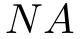
\includegraphics[width=22.60pt]{images-full/p247-i001.png}}\allowbreak{} 的参数方程为
\sourceblock{162.15}{images-full/p247-d001.png}
\sourceblock{306.23}{images-full/p247-d002.png}
\sourceblock{300.58}{images-full/p247-d003.png}
从而可得点\allowbreak{}\raisebox{-2.64pt}{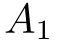
\includegraphics[width=15.82pt]{images-full/p247-i002.png}}\allowbreak{}的坐标为
\sourceblock{222.04}{images-full/p247-d004.png}
同理可得点\allowbreak{}\raisebox{-2.64pt}{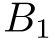
\includegraphics[width=15.25pt]{images-full/p247-i003.png}}\allowbreak{}的坐标为
\sourceblock{207.35}{images-full/p247-d005.png}
以及点\allowbreak{}\raisebox{-2.64pt}{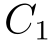
\includegraphics[width=15.25pt]{images-full/p247-i004.png}}\allowbreak{} 的坐标为
\sourceblock{207.35}{images-full/p247-d006.png}
\sourceblock{450.00}{images-full/p247-d007.png}
\sourceblock{304.53}{images-full/p247-d008.png}


% SOURCE_PDF_PAGE 248

\hypertarget{source-p248}{}
\par\medskip\noindent\textbf{【例5.2.14 】求过点\allowbreak{}\raisebox{-3.00pt}{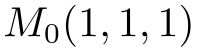
\includegraphics[width=55.93pt]{images-full/p248-i000.png}}\allowbreak{} 且与直线}
\sourceblock{127.12}{images-full/p248-d000.png}
\sourceblock{294.93}{images-full/p248-d001.png}
都相交的直线方程.
解(方法1) \allowbreak{}\raisebox{-2.64pt}{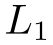
\includegraphics[width=14.69pt]{images-full/p248-i001.png}}\allowbreak{}经过\allowbreak{}\raisebox{-3.00pt}{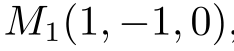
\includegraphics[width=65.84pt]{images-full/p248-i002.png}}\allowbreak{}，方向向量为\allowbreak{}\raisebox{-3.00pt}{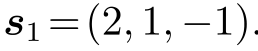
\includegraphics[width=72.74pt]{images-full/p248-i003.png}}\allowbreak{} \allowbreak{}\raisebox{-2.64pt}{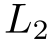
\includegraphics[width=15.25pt]{images-full/p248-i004.png}}\allowbreak{} 经过\allowbreak{}\raisebox{-3.00pt}{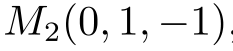
\includegraphics[width=65.56pt]{images-full/p248-i005.png}}\allowbreak{},
方向向量为\allowbreak{}\raisebox{-3.00pt}{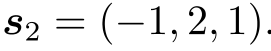
\includegraphics[width=76.21pt]{images-full/p248-i006.png}}\allowbreak{} 设所求直线方程为
\sourceblock{146.90}{images-full/p248-d002.png}
\sourceblock{306.79}{images-full/p248-d003.png}
\sourceblock{274.59}{images-full/p248-d004.png}
\sourceblock{127.12}{images-full/p248-d005.png}
\sourceblock{290.41}{images-full/p248-d006.png}
(方法2) 设所求直线与己知直线\allowbreak{}\raisebox{-2.64pt}{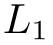
\includegraphics[width=14.69pt]{images-full/p248-i007.png}}\allowbreak{}以及\allowbreak{}\raisebox{-2.64pt}{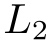
\includegraphics[width=15.25pt]{images-full/p248-i008.png}}\allowbreak{}分别交于\allowbreak{}\raisebox{-3.00pt}{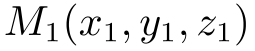
\includegraphics[width=71.75pt]{images-full/p248-i009.png}}\allowbreak{}与\allowbreak{}\raisebox{-3.00pt}{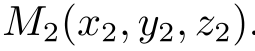
\includegraphics[width=71.68pt]{images-full/p248-i010.png}}\allowbreak{}'
\sourceblock{309.05}{images-full/p248-d007.png}
\sourceblock{308.49}{images-full/p248-d008.png}
其中\allowbreak{}\raisebox{-2.52pt}{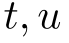
\includegraphics[width=19.21pt]{images-full/p248-i011.png}}\allowbreak{}也分别是参数，则\allowbreak{}\raisebox{-2.64pt}{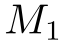
\includegraphics[width=18.08pt]{images-full/p248-i012.png}}\allowbreak{}与\allowbreak{}\raisebox{-2.64pt}{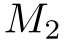
\includegraphics[width=18.64pt]{images-full/p248-i013.png}}\allowbreak{}点分别可以写作\allowbreak{}\raisebox{-3.00pt}{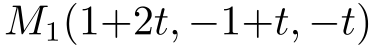
\includegraphics[width=105.65pt]{images-full/p248-i014.png}}\allowbreak{} 以及\allowbreak{}\raisebox{-3.00pt}{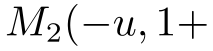
\includegraphics[width=59.89pt]{images-full/p248-i015.png}}\allowbreak{}
\allowbreak{}\raisebox{-3.00pt}{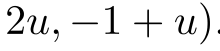
\includegraphics[width=61.94pt]{images-full/p248-i016.png}}\allowbreak{} 既然\allowbreak{}\raisebox{-3.00pt}{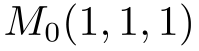
\includegraphics[width=55.93pt]{images-full/p248-i017.png}}\allowbreak{}在所求直线$L$上，则
\sourceblock{377.98}{images-full/p248-d009.png}


% SOURCE_PDF_PAGE 249

\hypertarget{source-p249}{}
\sourceblock{279.67}{images-full/p249-d000.png}
\sourceblock{450.00}{images-full/p249-d001.png}
可得过两点Mo ，M1 的直线L 的方程
\sourceblock{124.86}{images-full/p249-d002.png}
\sourceblock{177.41}{images-full/p249-d003.png}
设经过点\allowbreak{}\raisebox{-3.00pt}{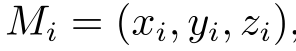
\includegraphics[width=83.35pt]{images-full/p249-i000.png}}\allowbreak{}，方向为\allowbreak{}\raisebox{-3.00pt}{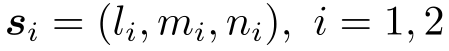
\includegraphics[width=126.56pt]{images-full/p249-i001.png}}\allowbreak{} 的两条直线
\sourceblock{163.85}{images-full/p249-d004.png}
\par\noindent (1) 直线\allowbreak{}\raisebox{-2.64pt}{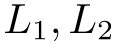
\includegraphics[width=33.33pt]{images-full/p249-i002.png}}\allowbreak{}之间的关系有如下四种情形: 平行、重合、相交和异面.{\symbolfont ①}当\allowbreak{}\raisebox{-3.00pt}{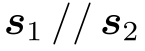
\includegraphics[width=40.68pt]{images-full/p249-i003.png}}\allowbreak{}
\sourceblock{450.00}{images-full/p249-d005.png}
\sourceblock{351.43}{images-full/p249-d006.png}
\par\noindent (3) 设\allowbreak{}\raisebox{-3.00pt}{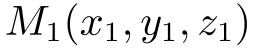
\includegraphics[width=71.75pt]{images-full/p249-i004.png}}\allowbreak{} 为空间中任意一点，则该点到直线
\sourceblock{158.76}{images-full/p249-d007.png}
\sourceblock{409.62}{images-full/p249-d008.png}


% SOURCE_PDF_PAGE 250

\hypertarget{source-p250}{}
\par\medskip\noindent\textbf{【例5.2.15 】求点\allowbreak{}\raisebox{-3.00pt}{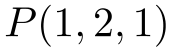
\includegraphics[width=48.59pt]{images-full/p250-i000.png}}\allowbreak{} 到直线}
\sourceblock{141.81}{images-full/p250-d000.png}
\sourceblock{450.00}{images-full/p250-d001.png}
另一方面，与$L$垂直的平面的法向量平行于直线$L$的方向向量，因此可以取\allowbreak{}\raisebox{-3.00pt}{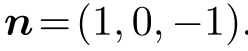
\includegraphics[width=69.64pt]{images-full/p250-i003.png}}\allowbreak{}
\sourceblock{280.24}{images-full/p250-d002.png}
即
\sourceblock{54.80}{images-full/p250-d003.png}
\par\medskip\noindent\textbf{【例5.2.16 】证明:如果直线}
\sourceblock{185.32}{images-full/p250-d004.png}
\sourceblock{314.14}{images-full/p250-d005.png}
\sourceblock{290.41}{images-full/p250-d006.png}
\par\noindent\textbf{证明}\ 经过\allowbreak{}\raisebox{-2.52pt}{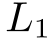
\includegraphics[width=14.69pt]{images-full/p250-i004.png}}\allowbreak{}的平面束为
\sourceblock{322.05}{images-full/p250-d007.png}


% SOURCE_PDF_PAGE 251

\hypertarget{source-p251}{}
其中\allowbreak{}\raisebox{-2.76pt}{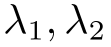
\includegraphics[width=31.07pt]{images-full/p251-i000.png}}\allowbreak{}为不全为零的任意实数.经过直线\allowbreak{}\raisebox{-2.52pt}{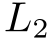
\includegraphics[width=15.25pt]{images-full/p251-i001.png}}\allowbreak{} 的平面束为
\sourceblock{322.05}{images-full/p251-d000.png}
其中\allowbreak{}\raisebox{-2.76pt}{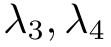
\includegraphics[width=31.07pt]{images-full/p251-i002.png}}\allowbreak{}为不全为零的任意实数. \allowbreak{}\raisebox{-2.64pt}{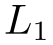
\includegraphics[width=14.69pt]{images-full/p251-i003.png}}\allowbreak{}与\allowbreak{}\raisebox{-2.64pt}{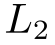
\includegraphics[width=15.25pt]{images-full/p251-i004.png}}\allowbreak{}共面，则存在非零常数$m$ 使得
\sourceblock{355.95}{images-full/p251-d001.png}
由上述恒等式，可得
\sourceblock{207.92}{images-full/p251-d002.png}
既然\allowbreak{}\raisebox{-2.76pt}{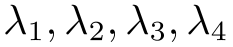
\includegraphics[width=65.54pt]{images-full/p251-i006.png}}\allowbreak{}不全为零，则有
\sourceblock{148.03}{images-full/p251-d003.png}
因为\allowbreak{}\raisebox{-2.88pt}{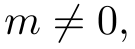
\includegraphics[width=37.85pt]{images-full/p251-i007.png}}\allowbreak{}，所以得
\sourceblock{371.20}{images-full/p251-d004.png}
\par\medskip\noindent\textbf{【例5.2.17】求\allowbreak{}\raisebox{-2.76pt}{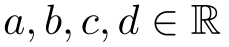
\includegraphics[width=64.41pt]{images-full/p251-i008.png}}\allowbreak{} 使得直线}
\sourceblock{147.46}{images-full/p251-d005.png}
\sourceblock{292.10}{images-full/p251-d006.png}
重合.


% SOURCE_PDF_PAGE 252

\hypertarget{source-p252}{}
\sourceblock{450.00}{images-full/p252-d000.png}
\sourceblock{118.08}{images-full/p252-d001.png}
于是解得\allowbreak{}\raisebox{-2.76pt}{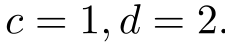
\includegraphics[width=63.31pt]{images-full/p252-i000.png}}\allowbreak{}.
\sourceblock{259.90}{images-full/p252-d002.png}
\sourceblock{163.85}{images-full/p252-d003.png}
\sourceblock{163.85}{images-full/p252-d004.png}
\sourceblock{262.16}{images-full/p252-d005.png}
\sourceblock{118.08}{images-full/p252-d006.png}
\par\noindent (3) 设\allowbreak{}\raisebox{-3.00pt}{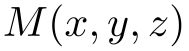
\includegraphics[width=53.11pt]{images-full/p252-i001.png}}\allowbreak{} 是直线\allowbreak{}\raisebox{-2.76pt}{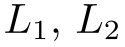
\includegraphics[width=35.03pt]{images-full/p252-i002.png}}\allowbreak{}公垂线上的任意一点，\allowbreak{}\raisebox{-2.04pt}{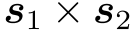
\includegraphics[width=38.42pt]{images-full/p252-i003.png}}\allowbreak{} 为公垂线的方向向量，
\sourceblock{291.54}{images-full/p252-d007.png}
\sourceblock{349.73}{images-full/p252-d008.png}


% SOURCE_PDF_PAGE 253

\hypertarget{source-p253}{}
\sourceblock{268.38}{images-full/p253-d000.png}
\sourceblock{296.62}{images-full/p253-d001.png}
之间的距离以及它们的公垂线方程.
\sourceblock{450.00}{images-full/p253-d002.png}
\sourceblock{348.60}{images-full/p253-d003.png}
于是可得\allowbreak{}\raisebox{-2.64pt}{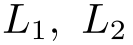
\includegraphics[width=37.29pt]{images-full/p253-i000.png}}\allowbreak{}之间的距离为
\sourceblock{170.63}{images-full/p253-d004.png}
记\allowbreak{}\raisebox{-3.00pt}{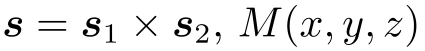
\includegraphics[width=119.78pt]{images-full/p253-i001.png}}\allowbreak{} 是直线\allowbreak{}\raisebox{-2.52pt}{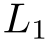
\includegraphics[width=13.56pt]{images-full/p253-i002.png}}\allowbreak{}与直线\allowbreak{}\raisebox{-2.64pt}{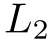
\includegraphics[width=15.25pt]{images-full/p253-i003.png}}\allowbreak{} 公垂线上的任意一点，则
\sourceblock{289.84}{images-full/p253-d005.png}
\sourceblock{308.49}{images-full/p253-d006.png}


% SOURCE_PDF_PAGE 254

\hypertarget{source-p254}{}
与平面
\sourceblock{145.77}{images-full/p254-d000.png}
之间的关系为以下三种情形.
\par\noindent (1) 相交:此时，\allowbreak{}\raisebox{-2.88pt}{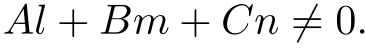
\includegraphics[width=102.91pt]{images-full/p254-i000.png}}\allowbreak{}
\par\noindent (2) 平行:此时，\allowbreak{}\raisebox{-2.76pt}{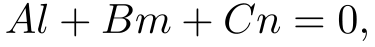
\includegraphics[width=105.65pt]{images-full/p254-i001.png}}\allowbreak{}，但\allowbreak{}\raisebox{-2.76pt}{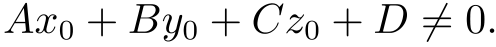
\includegraphics[width=140.00pt]{images-full/p254-i002.png}}\allowbreak{}
\sourceblock{346.91}{images-full/p254-d001.png}
\sourceblock{335.04}{images-full/p254-d002.png}
\sourceblock{311.88}{images-full/p254-d003.png}
与平面
\sourceblock{145.77}{images-full/p254-d004.png}
的三种关系对应于线性方程组
\sourceblock{311.88}{images-full/p254-d005.png}
的以下三种情形:
\par\noindent (1) 直线$L$与平面\allowbreak{}\raisebox{-1.56pt}{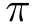
\includegraphics[width=10.17pt]{images-full/p254-i004.png}}\allowbreak{}相交，则方程组(5.2.8) 有唯一解，此时
\sourceblock{329.39}{images-full/p254-d006.png}
\sourceblock{269.50}{images-full/p254-d007.png}


% SOURCE_PDF_PAGE 255

\hypertarget{source-p255}{}
\par\noindent (3) 直线$L$与平面\allowbreak{}\raisebox{-1.56pt}{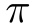
\includegraphics[width=10.17pt]{images-full/p255-i001.png}}\allowbreak{}重合，则方程组(5.2.8) 有无穷多解，此时
\sourceblock{289.84}{images-full/p255-d000.png}
\par\medskip\noindent\textbf{【例5.2.19 】求过直线}
\sourceblock{142.38}{images-full/p255-d001.png}
\sourceblock{277.98}{images-full/p255-d002.png}
垂直的平面方程.
解直线$L$ 由两个平面的交线构成，我们设过两个平面的平面束为
\sourceblock{222.61}{images-full/p255-d003.png}
整理可得
\sourceblock{251.99}{images-full/p255-d004.png}
因为平面柬与平面\allowbreak{}\raisebox{-2.76pt}{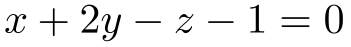
\includegraphics[width=98.87pt]{images-full/p255-i003.png}}\allowbreak{}垂直，所以有
\sourceblock{208.48}{images-full/p255-d005.png}
可得\allowbreak{}\raisebox{-2.88pt}{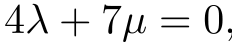
\includegraphics[width=65.21pt]{images-full/p255-i004.png}}\allowbreak{}，代入平面束方程可得所求平面方程
\sourceblock{119.21}{images-full/p255-d006.png}
\par\medskip\noindent\textbf{【例5.2.20 】求过点\allowbreak{}\raisebox{-3.00pt}{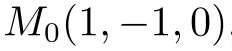
\includegraphics[width=65.44pt]{images-full/p255-i005.png}}\allowbreak{}，与平面}
\sourceblock{125.43}{images-full/p255-d007.png}
\sourceblock{450.00}{images-full/p255-d008.png}


% SOURCE_PDF_PAGE 256

\hypertarget{source-p256}{}
它与己知直线$L$相交.下面求交点.设
\sourceblock{124.30}{images-full/p256-d000.png}
\sourceblock{450.00}{images-full/p256-d001.png}
\sourceblock{104.52}{images-full/p256-d002.png}
(方法2) 设过\allowbreak{}\raisebox{-3.00pt}{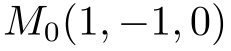
\includegraphics[width=64.97pt]{images-full/p256-i001.png}}\allowbreak{} 点的直线方程为
\sourceblock{450.00}{images-full/p256-d003.png}
\sourceblock{119.21}{images-full/p256-d004.png}
\sourceblock{284.76}{images-full/p256-d005.png}
\par\medskip\noindent\textbf{【例5.2.21 】(第十二届全国初赛题)己知椭球面}
\sourceblock{154.24}{images-full/p256-d006.png}
的外切柱面\allowbreak{}\raisebox{-3.00pt}{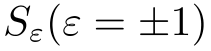
\includegraphics[width=59.32pt]{images-full/p256-i002.png}}\allowbreak{} 平行于已知直线
\sourceblock{176.84}{images-full/p256-d007.png}
试求与\allowbreak{}\raisebox{-2.76pt}{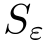
\includegraphics[width=13.56pt]{images-full/p256-i003.png}}\allowbreak{}交于一个圆周的平面的法方向.


% SOURCE_PDF_PAGE 257

\hypertarget{source-p257}{}
【注5.2.2 】本题中的外切柱面指的是每一条直母线均与己知椭球面相切的柱面.
解设$L$ 是柱面的任意一条直母钱，则由假设，$L$ 与己知椭球面\allowbreak{}\raisebox{-2.64pt}{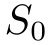
\includegraphics[width=14.69pt]{images-full/p257-i002.png}}\allowbreak{} 相切于一点
\allowbreak{}\raisebox{-3.00pt}{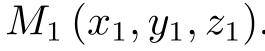
\includegraphics[width=74.41pt]{images-full/p257-i003.png}}\allowbreak{} 因为$L$平行于己知直线\allowbreak{}\raisebox{-2.64pt}{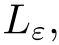
\includegraphics[width=16.31pt]{images-full/p257-i005.png}}\allowbreak{} 所以，$L$ 的标准方程和参数方程分别是
\sourceblock{410.19}{images-full/p257-d000.png}
\sourceblock{373.46}{images-full/p257-d001.png}
\sourceblock{397.76}{images-full/p257-d002.png}
联立解出
\sourceblock{361.03}{images-full/p257-d003.png}
再把\allowbreak{}\raisebox{-1.92pt}{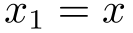
\includegraphics[width=37.29pt]{images-full/p257-i007.png}}\allowbreak{}和上面的两式代入\allowbreak{}\raisebox{-2.76pt}{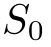
\includegraphics[width=14.12pt]{images-full/p257-i008.png}}\allowbreak{}的方程，得到外切柱面\allowbreak{}\raisebox{-2.76pt}{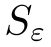
\includegraphics[width=14.12pt]{images-full/p257-i009.png}}\allowbreak{} 的方程为
\sourceblock{450.00}{images-full/p257-d004.png}
由于与二次柱面\allowbreak{}\raisebox{-2.76pt}{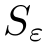
\includegraphics[width=13.56pt]{images-full/p257-i010.png}}\allowbreak{} 的交钱为圆周的所有平面都是平行的，故知所求的法方向唯一且为
\allowbreak{}\raisebox{-2.88pt}{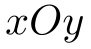
\includegraphics[width=25.42pt]{images-full/p257-i011.png}}\allowbreak{}平面的法方向\allowbreak{}\raisebox{-3.00pt}{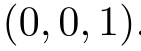
\includegraphics[width=39.73pt]{images-full/p257-i012.png}}\allowbreak{}


% SOURCE_PDF_PAGE 258

\hypertarget{source-p258}{}
\sourceblock{258.20}{images-full/p258-d000.png}
\sourceblock{281.93}{images-full/p258-d001.png}
的平面方程.
解(方法1) 设所求平面的法向量\allowbreak{}\raisebox{-3.00pt}{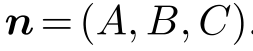
\includegraphics[width=71.16pt]{images-full/p258-i000.png}}\allowbreak{} 由题设可知直线\allowbreak{}\raisebox{-2.64pt}{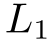
\includegraphics[width=14.69pt]{images-full/p258-i001.png}}\allowbreak{} 的方向\allowbreak{}\raisebox{-2.04pt}{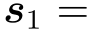
\includegraphics[width=25.99pt]{images-full/p258-i002.png}}\allowbreak{}
\allowbreak{}\raisebox{-3.00pt}{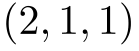
\includegraphics[width=38.98pt]{images-full/p258-i003.png}}\allowbreak{} 与直线\allowbreak{}\raisebox{-2.64pt}{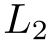
\includegraphics[width=15.25pt]{images-full/p258-i004.png}}\allowbreak{} 的方向\allowbreak{}\raisebox{-3.00pt}{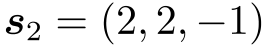
\includegraphics[width=75.71pt]{images-full/p258-i005.png}}\allowbreak{} 均与$n$ 垂直，即\allowbreak{}\raisebox{-2.64pt}{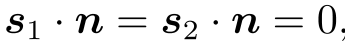
\includegraphics[width=97.18pt]{images-full/p258-i007.png}}\allowbreak{}，于是
\sourceblock{104.52}{images-full/p258-d002.png}
\sourceblock{450.00}{images-full/p258-d003.png}
\sourceblock{284.76}{images-full/p258-d004.png}
(方法2) 由题设可知，所求平面与直线\allowbreak{}\raisebox{-2.64pt}{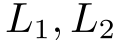
\includegraphics[width=33.90pt]{images-full/p258-i008.png}}\allowbreak{}均垂直，所以所求平面的法向量可设
为\allowbreak{}\raisebox{-2.88pt}{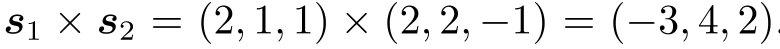
\includegraphics[width=220.11pt]{images-full/p258-i009.png}}\allowbreak{} 又因为直线\allowbreak{}\raisebox{-2.64pt}{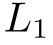
\includegraphics[width=14.69pt]{images-full/p258-i010.png}}\allowbreak{}上的点\allowbreak{}\raisebox{-2.88pt}{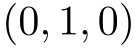
\includegraphics[width=38.98pt]{images-full/p258-i011.png}}\allowbreak{} 在所求平
\sourceblock{323.74}{images-full/p258-d005.png}
\sourceblock{284.19}{images-full/p258-d006.png}
\par\medskip\noindent\textbf{【例5.2.23 】求过点\allowbreak{}\raisebox{-3.00pt}{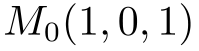
\includegraphics[width=55.93pt]{images-full/p258-i012.png}}\allowbreak{} 和直线}
\sourceblock{144.07}{images-full/p258-d007.png}
的平面方程.
解直线$L$ 的方向向量为\allowbreak{}\raisebox{-3.00pt}{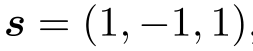
\includegraphics[width=71.27pt]{images-full/p258-i014.png}}\allowbreak{}，因为直线$L$上的点\allowbreak{}\raisebox{-3.00pt}{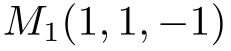
\includegraphics[width=64.97pt]{images-full/p258-i016.png}}\allowbreak{} 也在所求
平面上，所以向\allowbreak{}\raisebox{-5.00pt}{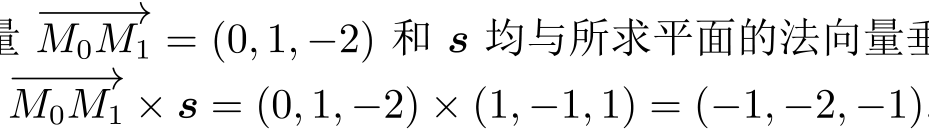
\includegraphics[width=262.30pt]{images-full/p258-i017.png}}\allowbreak{}直，因此所求平面的
法向量可以设为 故所求平面为
\sourceblock{179.10}{images-full/p258-d008.png}
\sourceblock{277.98}{images-full/p258-d009.png}


% SOURCE_PDF_PAGE 259

\hypertarget{source-p259}{}
\phantomsection\addcontentsline{toc}{section}{5.3 真题选讲与点评}
\par 作.3真题选讲与点评)
\par\medskip\noindent\textbf{【例5.3.1 】(第三届全国决赛题)设有空间中的五点}
\sourceblock{327.70}{images-full/p259-d000.png}
试求过点$E$且与\allowbreak{}\raisebox{-2.76pt}{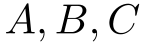
\includegraphics[width=41.24pt]{images-full/p259-i001.png}}\allowbreak{}所在平面\allowbreak{}\raisebox{-1.56pt}{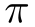
\includegraphics[width=9.60pt]{images-full/p259-i002.png}}\allowbreak{}平行而与直线\allowbreak{}\raisebox{-2.28pt}{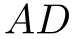
\includegraphics[width=21.47pt]{images-full/p259-i003.png}}\allowbreak{} 垂直的直线方程.
解平面\allowbreak{}\raisebox{-2.40pt}{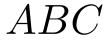
\includegraphics[width=30.51pt]{images-full/p259-i004.png}}\allowbreak{} 的法向量
\sourceblock{267.24}{images-full/p259-d001.png}
设所求直线的方向向量为\allowbreak{}\raisebox{-3.00pt}{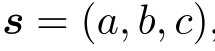
\includegraphics[width=60.48pt]{images-full/p259-i005.png}}\allowbreak{}，则由题设条件可得
\sourceblock{131.08}{images-full/p259-d002.png}
由此解得\allowbreak{}\raisebox{-3.00pt}{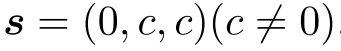
\includegraphics[width=96.04pt]{images-full/p259-i006.png}}\allowbreak{} 取\allowbreak{}\raisebox{-3.00pt}{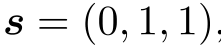
\includegraphics[width=62.11pt]{images-full/p259-i007.png}}\allowbreak{}，于是得到所求直线方程为
\sourceblock{124.86}{images-full/p259-d003.png}
\par\medskip\noindent\textbf{【例5.3.2】(第六届全国初赛题)己知空间的两条直线}
\sourceblock{308.49}{images-full/p259-d004.png}
\par\noindent (1) 证明\allowbreak{}\raisebox{-2.52pt}{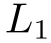
\includegraphics[width=14.12pt]{images-full/p259-i008.png}}\allowbreak{}和\allowbreak{}\raisebox{-2.52pt}{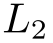
\includegraphics[width=14.69pt]{images-full/p259-i009.png}}\allowbreak{} 异面;
\par\noindent (2) 求\allowbreak{}\raisebox{-2.64pt}{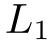
\includegraphics[width=14.69pt]{images-full/p259-i010.png}}\allowbreak{}和\allowbreak{}\raisebox{-2.64pt}{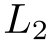
\includegraphics[width=14.69pt]{images-full/p259-i011.png}}\allowbreak{} 公垂线的标准方程;
\par\noindent (3) 求连接\allowbreak{}\raisebox{-2.64pt}{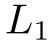
\includegraphics[width=14.69pt]{images-full/p259-i012.png}}\allowbreak{}上的任一点和\allowbreak{}\raisebox{-2.64pt}{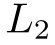
\includegraphics[width=15.25pt]{images-full/p259-i013.png}}\allowbreak{}上的任一点线段中点的轨迹的一般方程.
\par\noindent (1) 证明显然，点\allowbreak{}\raisebox{-3.00pt}{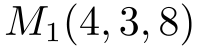
\includegraphics[width=55.93pt]{images-full/p259-i014.png}}\allowbreak{} 在直线\allowbreak{}\raisebox{-2.64pt}{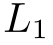
\includegraphics[width=14.69pt]{images-full/p259-i015.png}}\allowbreak{}上，\allowbreak{}\raisebox{-3.00pt}{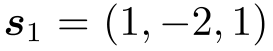
\includegraphics[width=76.84pt]{images-full/p259-i016.png}}\allowbreak{} 为\allowbreak{}\raisebox{-2.64pt}{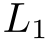
\includegraphics[width=14.69pt]{images-full/p259-i017.png}}\allowbreak{}的方向向量.叉
点\allowbreak{}\raisebox{-3.00pt}{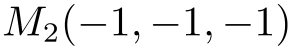
\includegraphics[width=83.05pt]{images-full/p259-i018.png}}\allowbreak{} 在直线\allowbreak{}\raisebox{-2.64pt}{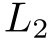
\includegraphics[width=15.25pt]{images-full/p259-i019.png}}\allowbreak{}上，\allowbreak{}\raisebox{-2.88pt}{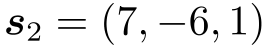
\includegraphics[width=75.71pt]{images-full/p259-i020.png}}\allowbreak{} 为\allowbreak{}\raisebox{-2.64pt}{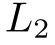
\includegraphics[width=15.25pt]{images-full/p259-i021.png}}\allowbreak{} 的方向向量.因为
\sourceblock{450.00}{images-full/p259-d005.png}
\allowbreak{}\raisebox{-2.64pt}{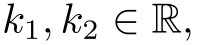
\includegraphics[width=55.72pt]{images-full/p259-i022.png}}\allowbreak{}，所以
\sourceblock{409.06}{images-full/p259-d006.png}


% SOURCE_PDF_PAGE 260

\hypertarget{source-p260}{}
又直线\allowbreak{}\raisebox{-2.52pt}{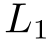
\includegraphics[width=14.12pt]{images-full/p260-i000.png}}\allowbreak{}和\allowbreak{}\raisebox{-2.52pt}{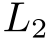
\includegraphics[width=14.69pt]{images-full/p260-i001.png}}\allowbreak{} 的公垂线的方向向量为
\sourceblock{263.29}{images-full/p260-d000.png}
故当\allowbreak{}\raisebox{-3.96pt}{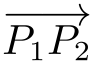
\includegraphics[width=27.12pt]{images-full/p260-i002.png}}\allowbreak{}与$s$ 平行时，直线\allowbreak{}\raisebox{-2.64pt}{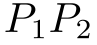
\includegraphics[width=27.12pt]{images-full/p260-i004.png}}\allowbreak{}就是\allowbreak{}\raisebox{-2.64pt}{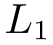
\includegraphics[width=14.69pt]{images-full/p260-i005.png}}\allowbreak{}和\allowbreak{}\raisebox{-2.64pt}{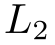
\includegraphics[width=15.25pt]{images-full/p260-i006.png}}\allowbreak{} 的公垂线，此时有
\par (-5+7问- k 1 ) : (-4 - 6k2 + 2k1 ) : (-9 + k2 - kt) = 2 : 3 : 4,
由此解得\allowbreak{}\raisebox{-2.64pt}{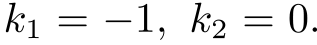
\includegraphics[width=89.20pt]{images-full/p260-i007.png}}\allowbreak{} 这表明，点\allowbreak{}\raisebox{-3.00pt}{\includegraphics[width=83.62pt]{images-full/p260-i008.png}}\allowbreak{} 与\allowbreak{}\raisebox{-2.64pt}{\includegraphics[width=14.69pt]{images-full/p260-i009.png}}\allowbreak{} 重合，点\allowbreak{}\raisebox{-2.64pt}{\includegraphics[width=18.08pt]{images-full/p260-i010.png}}\allowbreak{} 在公垂线上，
\sourceblock{290.41}{images-full/p260-d001.png}
\par\noindent (3) 解对任意点\allowbreak{}\raisebox{-2.64pt}{\includegraphics[width=92.66pt]{images-full/p260-i011.png}}\allowbreak{} 根据\allowbreak{}\raisebox{-2.64pt}{\includegraphics[width=14.12pt]{images-full/p260-i012.png}}\allowbreak{}和\allowbreak{}\raisebox{-2.64pt}{\includegraphics[width=15.25pt]{images-full/p260-i013.png}}\allowbreak{} 的参数方程，易知$R$与\allowbreak{}\raisebox{-2.64pt}{\includegraphics[width=14.12pt]{images-full/p260-i015.png}}\allowbreak{}的坐
标为\allowbreak{}\raisebox{-3.00pt}{\includegraphics[width=269.72pt]{images-full/p260-i016.png}}\allowbreak{}，其中\allowbreak{}\raisebox{-2.76pt}{\includegraphics[width=49.65pt]{images-full/p260-i017.png}}\allowbreak{}，由此可知线段
\allowbreak{}\raisebox{-2.64pt}{\includegraphics[width=27.68pt]{images-full/p260-i018.png}}\allowbreak{} 的中点的坐标为
\sourceblock{215.26}{images-full/p260-d002.png}
\sourceblock{450.00}{images-full/p260-d003.png}
\par\medskip\noindent\textbf{【例5.3.31 (第七届全国初赛题)设\allowbreak{}\raisebox{-2.64pt}{\includegraphics[width=14.69pt]{images-full/p260-i019.png}}\allowbreak{} 和\allowbreak{}\raisebox{-2.64pt}{\includegraphics[width=14.69pt]{images-full/p260-i020.png}}\allowbreak{} 是空间中的两条异面直线，且在标准}
直角坐标系下直线\allowbreak{}\raisebox{-2.64pt}{\includegraphics[width=14.69pt]{images-full/p260-i021.png}}\allowbreak{}过坐标为\allowbreak{}\raisebox{-1.68pt}{\includegraphics[width=8.47pt]{images-full/p260-i022.png}}\allowbreak{} 的点，以单位向量\allowbreak{}\raisebox{-1.68pt}{\includegraphics[width=9.60pt]{images-full/p260-i023.png}}\allowbreak{}为直线方向;直线\allowbreak{}\raisebox{-2.64pt}{\includegraphics[width=15.25pt]{images-full/p260-i024.png}}\allowbreak{} 过坐标为$b$
的点，以单位向量\allowbreak{}\raisebox{-1.68pt}{\includegraphics[width=12.43pt]{images-full/p260-i026.png}}\allowbreak{} 为直线方向
\par\noindent (1) 证明:存在唯一点\allowbreak{}\raisebox{-2.64pt}{\includegraphics[width=37.85pt]{images-full/p260-i027.png}}\allowbreak{}和\allowbreak{}\raisebox{-2.76pt}{\includegraphics[width=38.98pt]{images-full/p260-i028.png}}\allowbreak{}使得两点连线\allowbreak{}\raisebox{-2.76pt}{\includegraphics[width=20.90pt]{images-full/p260-i029.png}}\allowbreak{} 同时垂直于\allowbreak{}\raisebox{-2.64pt}{\includegraphics[width=14.69pt]{images-full/p260-i030.png}}\allowbreak{}和\allowbreak{}\raisebox{-2.64pt}{\includegraphics[width=15.55pt]{images-full/p260-i031.png}}\allowbreak{}.
\par\noindent (2) 求$P$ 点和$Q$ 点的坐标(用\allowbreak{}\raisebox{-2.76pt}{\includegraphics[width=46.89pt]{images-full/p260-i034.png}}\allowbreak{}表示).
\par\noindent (1) 证明根据题设，\allowbreak{}\raisebox{-2.64pt}{\includegraphics[width=14.69pt]{images-full/p260-i035.png}}\allowbreak{}和\allowbreak{}\raisebox{-2.64pt}{\includegraphics[width=15.25pt]{images-full/p260-i036.png}}\allowbreak{}是异面直线，所以\allowbreak{}\raisebox{-2.76pt}{\includegraphics[width=57.03pt]{images-full/p260-i037.png}}\allowbreak{} 过直线\allowbreak{}\raisebox{-2.64pt}{\includegraphics[width=14.69pt]{images-full/p260-i038.png}}\allowbreak{}上一点并以
\allowbreak{}\raisebox{-1.80pt}{\includegraphics[width=34.46pt]{images-full/p260-i039.png}}\allowbreak{}为法向量作平面\allowbreak{}\raisebox{-2.04pt}{\includegraphics[width=12.43pt]{images-full/p260-i040.png}}\allowbreak{}则直线\allowbreak{}\raisebox{-2.64pt}{\includegraphics[width=14.69pt]{images-full/p260-i041.png}}\allowbreak{} 落在平面\allowbreak{}\raisebox{-1.68pt}{\includegraphics[width=9.60pt]{images-full/p260-i042.png}}\allowbreak{}上，且直线\allowbreak{}\raisebox{-2.64pt}{\includegraphics[width=14.69pt]{images-full/p260-i043.png}}\allowbreak{} 平行于平面\allowbreak{}\raisebox{-1.68pt}{\includegraphics[width=9.90pt]{images-full/p260-i044.png}}\allowbreak{} 又过\allowbreak{}\raisebox{-2.64pt}{\includegraphics[width=15.25pt]{images-full/p260-i045.png}}\allowbreak{}
作平面$T$垂直于平面\allowbreak{}\raisebox{-2.04pt}{\includegraphics[width=12.21pt]{images-full/p260-i047.png}}\allowbreak{}，记两个平面的交钱为\allowbreak{}\raisebox{-2.64pt}{\includegraphics[width=16.35pt]{images-full/p260-i048.png}}\allowbreak{} 设直线\allowbreak{}\raisebox{-2.64pt}{\includegraphics[width=15.25pt]{images-full/p260-i049.png}}\allowbreak{}和\allowbreak{}\raisebox{-2.64pt}{\includegraphics[width=14.69pt]{images-full/p260-i050.png}}\allowbreak{} 的交点为\allowbreak{}\raisebox{-2.64pt}{\includegraphics[width=13.13pt]{images-full/p260-i051.png}}\allowbreak{}过$P$ 作
\sourceblock{450.00}{images-full/p260-d004.png}


% SOURCE_PDF_PAGE 261

\hypertarget{source-p261}{}
\phantomsection\addcontentsline{toc}{section}{5.4 能力拓展与训练}
\sourceblock{393.80}{images-full/p261-d000.png}
\sourceblock{150.29}{images-full/p261-d001.png}
\sourceblock{389.28}{images-full/p261-d002.png}
\sourceblock{385.33}{images-full/p261-d003.png}
因此
\sourceblock{379.68}{images-full/p261-d004.png}
\sourceblock{320.92}{images-full/p261-d005.png}
\sourceblock{450.00}{images-full/p261-d006.png}
2. 己知直线
\sourceblock{450.00}{images-full/p261-d007.png}
4. 己知空间\allowbreak{}\raisebox{-1.68pt}{\includegraphics[width=9.60pt]{images-full/p261-i000.png}}\allowbreak{} 边形\allowbreak{}\raisebox{-2.76pt}{\includegraphics[width=62.71pt]{images-full/p261-i001.png}}\allowbreak{} 的边\allowbreak{}\raisebox{-2.88pt}{\includegraphics[width=120.34pt]{images-full/p261-i002.png}}\allowbreak{}，其中\allowbreak{}\raisebox{-2.88pt}{\includegraphics[width=64.41pt]{images-full/p261-i003.png}}\allowbreak{})所
在的直线与一个平面分别相交于点鸟\allowbreak{}\raisebox{-2.76pt}{\includegraphics[width=14.09pt]{images-full/p261-i004.png}}\allowbreak{}证明:
\sourceblock{167.24}{images-full/p261-d008.png}
\sourceblock{450.00}{images-full/p261-d009.png}


% SOURCE_PDF_PAGE 262

\hypertarget{source-p262}{}
\phantomsection\addcontentsline{toc}{section}{5.5 训练全解与分析}
\sourceblock{450.00}{images-full/p262-d000.png}
\sourceblock{320.92}{images-full/p262-d001.png}
\sourceblock{335.61}{images-full/p262-d002.png}
\sourceblock{250.86}{images-full/p262-d003.png}
困为点\allowbreak{}\raisebox{-2.88pt}{\includegraphics[width=67.23pt]{images-full/p262-i000.png}}\allowbreak{} 在平面\allowbreak{}\raisebox{-2.88pt}{\includegraphics[width=124.86pt]{images-full/p262-i001.png}}\allowbreak{}上，所以
\sourceblock{450.00}{images-full/p262-d004.png}
\allowbreak{}\raisebox{-3.00pt}{\includegraphics[width=149.40pt]{images-full/p262-i002.png}}\allowbreak{}，困为\allowbreak{}\raisebox{-2.04pt}{\includegraphics[width=12.43pt]{images-full/p262-i003.png}}\allowbreak{} 与\allowbreak{}\raisebox{-2.04pt}{\includegraphics[width=12.99pt]{images-full/p262-i004.png}}\allowbreak{} 不共线，所以两条直线共面当且仅当混合积


% SOURCE_PDF_PAGE 263

\hypertarget{source-p263}{}
\sourceblock{270.63}{images-full/p263-d000.png}
\sourceblock{387.02}{images-full/p263-d001.png}
\sourceblock{176.28}{images-full/p263-d002.png}
\sourceblock{450.00}{images-full/p263-d003.png}
\sourceblock{300.01}{images-full/p263-d004.png}
\sourceblock{290.97}{images-full/p263-d005.png}
(方法2) 所求直线可看作两个平面的交线，其一由己知点与第一条直线确定的平面，
其二由己知点与第二条直线确定的平面，所以
\sourceblock{286.45}{images-full/p263-d006.png}
\sourceblock{450.00}{images-full/p263-d007.png}
\sourceblock{278.54}{images-full/p263-d008.png}


% SOURCE_PDF_PAGE 264

\hypertarget{source-p264}{}
因此得
\sourceblock{320.35}{images-full/p264-d000.png}
\sourceblock{303.97}{images-full/p264-d001.png}
\sourceblock{175.71}{images-full/p264-d002.png}
\sourceblock{450.00}{images-full/p264-d003.png}
\sourceblock{180.23}{images-full/p264-d004.png}
\sourceblock{237.30}{images-full/p264-d005.png}
\sourceblock{297.75}{images-full/p264-d006.png}
\sourceblock{397.19}{images-full/p264-d007.png}
6. 解引入经过点$A$ 且与直线$L$垂直的辅助平面$M$，即图5.4.1 中的\allowbreak{}\raisebox{-2.40pt}{\includegraphics[width=29.94pt]{images-full/p264-i003.png}}\allowbreak{} 平面.
因为直线$L$ 的方向向量\allowbreak{}\raisebox{-3.00pt}{\includegraphics[width=63.34pt]{images-full/p264-i005.png}}\allowbreak{}，所以平面$M$ 的方程为
\sourceblock{225.43}{images-full/p264-d008.png}
\sourceblock{450.00}{images-full/p264-d009.png}


% SOURCE_PDF_PAGE 265

\hypertarget{source-p265}{}
\sourceblock{167.80}{images-full/p265-d000.png}
圄5.4.1
\sourceblock{432.79}{images-full/p265-d001.png}
\allowbreak{}\raisebox{-2.88pt}{\includegraphics[width=33.00pt]{images-full/p265-i000.png}}\allowbreak{}, \allowbreak{}\raisebox{-3.00pt}{\includegraphics[width=75.35pt]{images-full/p265-i001.png}}\allowbreak{}，因为
\sourceblock{244.08}{images-full/p265-d002.png}
所以公垂线的方向向量可取为\allowbreak{}\raisebox{-2.88pt}{\includegraphics[width=70.86pt]{images-full/p265-i002.png}}\allowbreak{}.
经过直线\allowbreak{}\raisebox{-2.64pt}{\includegraphics[width=14.12pt]{images-full/p265-i003.png}}\allowbreak{}且平行于$s$ 的平面，经过直线\allowbreak{}\raisebox{-2.64pt}{\includegraphics[width=14.69pt]{images-full/p265-i005.png}}\allowbreak{}且平行于$s$ 的平面方程分别为
\sourceblock{290.41}{images-full/p265-d003.png}
\sourceblock{339.56}{images-full/p265-d004.png}
\sourceblock{359.34}{images-full/p265-d005.png}
\sourceblock{124.86}{images-full/p265-d006.png}
\sourceblock{303.97}{images-full/p265-d007.png}
\sourceblock{124.86}{images-full/p265-d008.png}


% SOURCE_PDF_PAGE 266

\hypertarget{source-p266}{}
\sourceblock{413.58}{images-full/p266-d000.png}
\sourceblock{450.00}{images-full/p266-d001.png}
\sourceblock{450.00}{images-full/p266-d002.png}
线$L$相交，因而共面，故由共面条件得
\sourceblock{163.28}{images-full/p266-d003.png}
即l\allowbreak{}\raisebox{-2.40pt}{\includegraphics[width=106.84pt]{images-full/p266-i001.png}}\allowbreak{} 与平面\allowbreak{}\raisebox{-2.52pt}{\includegraphics[width=94.35pt]{images-full/p266-i002.png}}\allowbreak{} 联立，得
\sourceblock{302.84}{images-full/p266-d004.png}
\sourceblock{450.00}{images-full/p266-d005.png}
则有3(-1)+4+λ=0，解得\allowbreak{}\raisebox{-2.28pt}{\includegraphics[width=40.91pt]{images-full/p266-i003.png}}\allowbreak{}.故叫:加一句+z-l = O. 另外，经过点A(-1, 0, 4)
\sourceblock{310.18}{images-full/p266-d006.png}


% SOURCE_PDF_PAGE 267

\hypertarget{source-p267}{}
即\allowbreak{}\raisebox{-2.76pt}{\includegraphics[width=122.09pt]{images-full/p267-i000.png}}\allowbreak{} 把它与平面\allowbreak{}\raisebox{-1.92pt}{\includegraphics[width=12.99pt]{images-full/p267-i001.png}}\allowbreak{}的方程联立即得所求直线的一般方程
\sourceblock{139.55}{images-full/p267-d000.png}
\sourceblock{450.00}{images-full/p267-d001.png}
\sourceblock{286.45}{images-full/p267-d002.png}
\sourceblock{358.77}{images-full/p267-d003.png}
\sourceblock{131.64}{images-full/p267-d004.png}
\sourceblock{432.79}{images-full/p267-d005.png}
151 与平面町的常数项D1 =-3 异号，而152 与平面町的常数项D2 =-1 同号，这表明
点\allowbreak{}\raisebox{-3.00pt}{\includegraphics[width=38.98pt]{images-full/p267-i002.png}}\allowbreak{} 与原点不在同一个二面角内.因此点\allowbreak{}\raisebox{-3.00pt}{\includegraphics[width=38.42pt]{images-full/p267-i003.png}}\allowbreak{} 所在的二面角的大小为
\sourceblock{90.96}{images-full/p267-d006.png}
